% Los anexos no tienen numeracion de seccion
\titleformat{\subsection}
	{\bfseries\large}
	{}
	{0.5pt}
	{}


\subsection{ANEXO I: Situaci�n actual de las empresas competidoras} \label{anexo:graficos}

\begin{figure}[!ht]
\centering
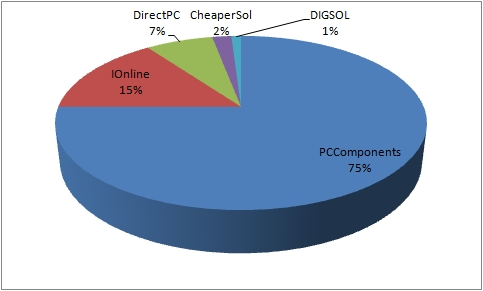
\includegraphics[scale=0.7,keepaspectratio]{./images/investigacion}%
\caption{Porcentaje de inversi�n en investigaci�n de nuevas tecnolog�as}%
\label{fig:factura}%
\end{figure}

\begin{figure}[!ht]
\centering
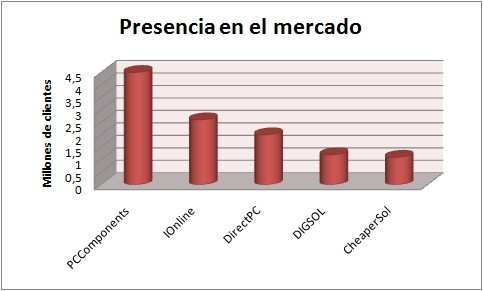
\includegraphics[scale=0.7,keepaspectratio]{./images/presencia}%
\caption{Presencia en el mercado de las empresas}%
\label{fig:factura}%
\end{figure}

\newpage
\subsection{ANEXO II: Organigrama de la empresa DIGSOL} \label{anexo:organigrama}

\begin{figure}[h]
\centering
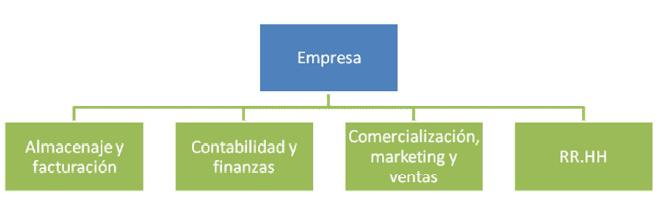
\includegraphics[scale=0.7,keepaspectratio]{./images/organigrama}%
\caption{Organigrama de la empresa DIGSOL}%
\label{fig:organigrama}%
\end{figure}


\subsection{ANEXO III: Adquisiciones tecnol�gicas} \label{anexo:facturas}

En la Figura \ref{fig:factura} se muestra una de las �ltimas adquisiciones tecnol�gicas de la empresa DIGSOL. En base a esa factura, se comentan los gastos que se encuentran innecesarios.

\begin{figure}[ht]
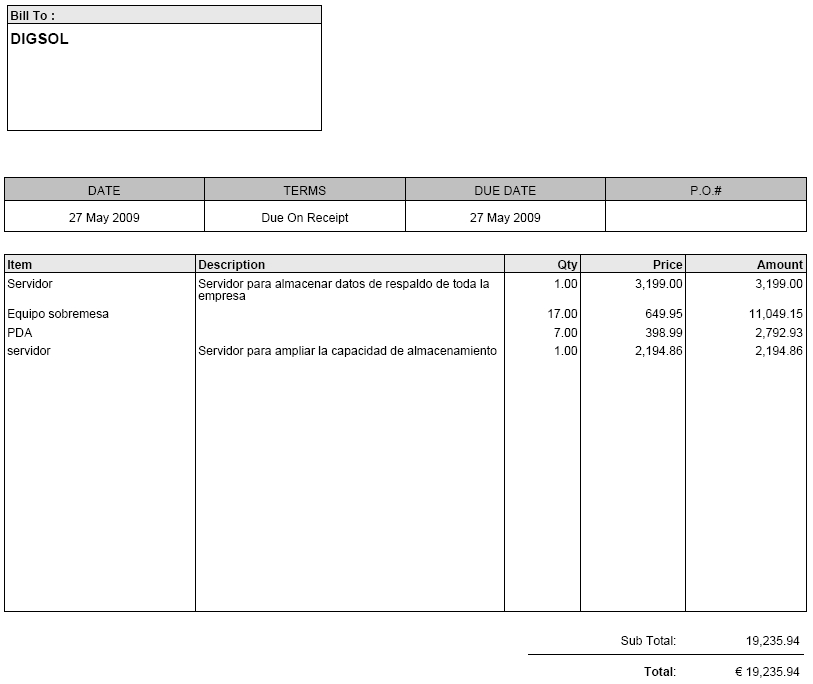
\includegraphics[scale=0.57,keepaspectratio]{./images/factura}%
\caption{Factura del 27-Mayo-2009}%
\label{fig:factura}%
\end{figure}

\begin{spacing}{1.4}

El servidor de respaldo es una adquisici�n necesaria, ya que la empresa no lo renovaba desde hace unos 3 o 4 a�os. Sin embargo, la compra de los 17 equipos de sobremesa, destinados al departamento de contabilidad de una de sus sedes, es algo innecesario, ya que pr�cticamente la totalidad de equipos de las diferentes sedes de la empresa se renovaron hace poco m�s de un a�o (coincidiendo con la implantaci�n del sistema Web), tal y como muestra la factura de esa �poca (ver Figura \ref{fig:facturaAntigua}).

\begin{figure}[ht]
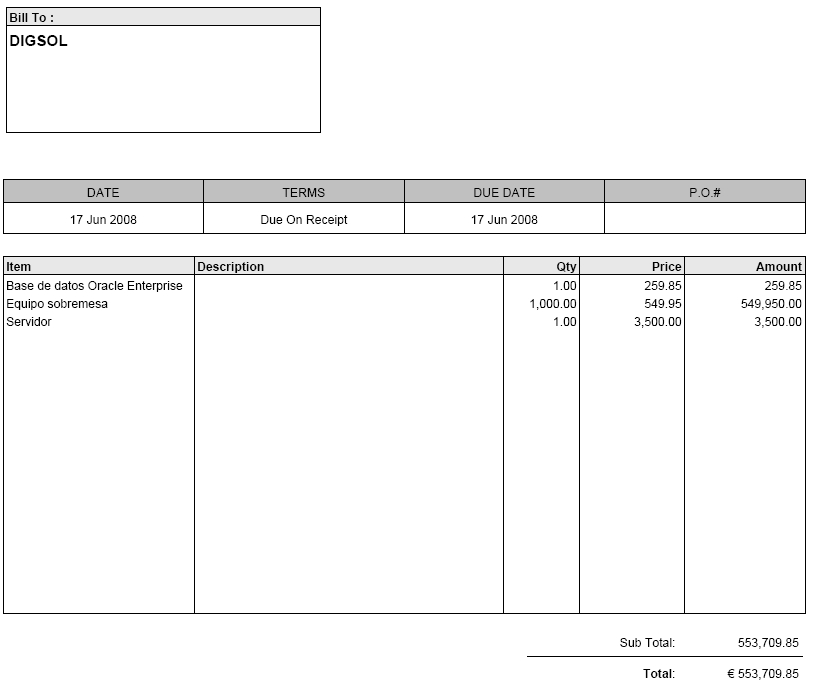
\includegraphics[scale=0.57,keepaspectratio]{./images/facturaAntigua}%
\caption{Fragmento de la factura del 17-Junio-2008}%
\label{fig:facturaAntigua}%
\end{figure}

Del mismo modo, adquirir un nuevo servidor para ampliar la capacidad de almacenamiento es, en el momento actual en el que se encuentra la empresa, algo innecsario, pues el servidor que se adquiri� en su dia tiene capacidad suficiente. Podr�a pensarse entonces en qu� es una adquisici�n �til para medio o largo plazo, pero esto no es as�, ya que las tecnolog�as avanzan r�pidamente y en un plazo relativamente corto, existir�n mejores soluciones en el mercado.


En lo que se refiere a la compra de las PDAs para las personas que integran el comit� de Direcci�n, es un gasto totalmente no justificado e in�til, ya que no se utilizan dichas PDAs para proporcionar valor al negocio. Podr�an aprovecharse para sincronizar los datos de la empresa en las PDAs, atender negocios en ella, etc., pero esto no ocurre as�.


\end{spacing}
